\section{Spectrometer Slit Systems}
\label{sec:slit}

\subsection{HMS}
\label{sssec:hms_slit}
The HMS slit system is installed on the gate valve housing mounted to the
front face of Q1. It consists of a vacuum box with a slit ladder
mounted into it. The slit ladder has space for three separate slits,
which will typically be one sieve slit and two solid angle defining collimators.
The slits are rectangular blocks of densimet (90\% W and 10\% Cu/Ni)
with a density of 17 g/cm$^3$. The collimators have an octagonal shaped
opening machined into them; the sieve slit has many holes drilled
into it.

The outer size of the collimators is 11.75" vertical by 8.25"
horizontal. The outer size of the sieve slit is 10.00" vertical
by 8.25" horizontal.
Its vertical size is reduced w.r.t. 11.75" due to space constraints.
The sieve slit always has to be installed at the bottom position of the ladder,
so that we can use the shielding of the collimator above it to
clearly distinguish the top row of holes. The central hole
of the sieve slit has a smaller aperture, and two blocked holes
exist to easily distinguish center and directions.
The collimator thicknesses are 2.5", while the sieve slit thickness
is 1.25". The dimensions and shape of the inner aperture of the present
HMS collimators is denoted in Table~\ref{tab:apertures}.

\begin{table}
\begin{center}
\caption{Apertures of Collimators\label{tab:apertures}}
%\vspace{\baselineskip}
\begin{tabular}{|c|c|c|c|c|}
\hline
{} & {} & {} & {} & {} \\
HMS & d$\Omega$ & Horizontal & Vertical & Shape \\
{}  & (msr) 	& (mr) 	     & (mr) 	& {} 	\\
{} & {} & {} & {} & {} \\ \hline
Large Collimator  & 6.74 & $\pm$ 27.5 	& $\pm$ 70.0 	& Octagonal, Flared 	\\
``Pion'' Collimator&  	& $\pm$	& $\pm$  	& Octagonal, Flared 	\\
{} & {} & {} & {} & {} \\ \hline
%SOS & 7.55 & $\pm$ 57.5 & $\pm$ 37.5 & Octagonal, Flared & \\
%SOS & 3.98 & $\pm$ 32.5 & $\pm$ 35.0 & Octagonal, Flared & \\
SHMS	& d$\Omega$ 	& Horizontal 	& Vertical 		& Shape 	\\
{} 	& (msr) 	& (mr) 		& (mr) 		& {} 	\\
Collimator &   4         & $\pm$ 24      &  $\pm$ 40     & Octagonal, Flared \\
\hline
\end{tabular}
\end{center}
\end{table}

The total depth of the slit box is close to 3.75", which leaves
enough space to later mount scintillators behind the collimators as an active
veto counter (to prevent punch-through of hadrons) and/or to increase
the collimator thickness. Two circular quick-connect flanges are
added for feed-through of possible light guides.

\subsection{SHMS}
\label{sssec:shms_slit}
A similar remotely-operated collimator box is installed on the SHMS between the
HB and Q1 magnets. The collimator ladder assembly within this box may be positioned
at three settings. The top position (accessed when the assembly is at its lowest
position) is a stretched octagon with opening height 9.843" and width 6.693" on the
upstream side. It is 2.5" thick. The lower two positions both present sieve holes in
rectangular pattern with holes separated by 0.6457" horizontally and 0.9843"
vertically. The sieve pattern at the middle ladder position has 11 columns of holes with
the sixth column centered horizontally. The holes on the bottom sieve are in ten
columns and are offset by one-half a column gap from those in the middle sieve.
The sieve collimators are 1.25" thick. The geometry is illustrated in Fig.~\ref{fig:SHMS_Collimators}.
Both sieves and octagonal collimator are
made of Mi-Tech\texttrademark{} Tungsten HD-17 (Density 17 g/cc. 90\%~W, 6\%~Ni, 4\%~Cu).

Because the SHMS has both a horizontal bend (HB magnet) and a vertical bend (main Dipole
magnet), a second sieve collimator is helpful for optics calibration and understanding the magnets.
It is placed immediately
upstream of the HB magnet entrance. Two options are provided: a conventional passive
sieve collimator and the so-called \textit{active sieve} which is a detector based on Gas Electron
Multipliers (GEMs).  A photo of the passive sieve options is shown in Fig.~\ref{fig:HB_Sieve_Photo}
and the dimensions and hole pattern are shown in Fig.~\ref{fig:HB_Sieve_Layout}.

\begin{figure}
\begin{center}
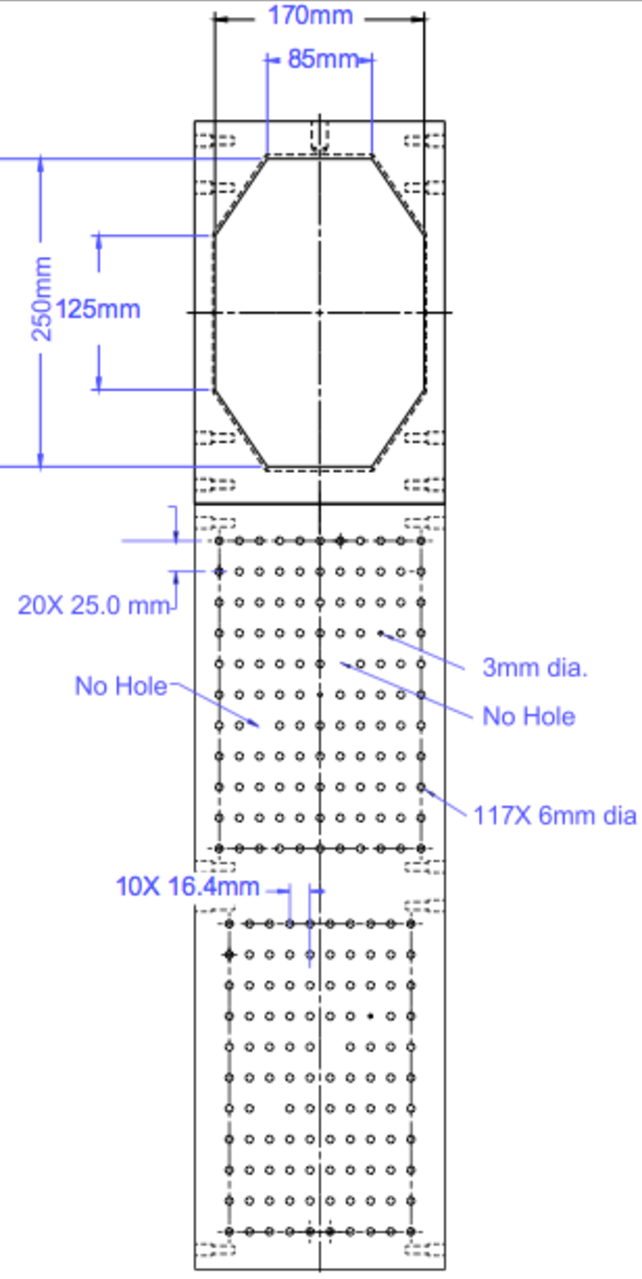
\includegraphics[width=2in]{SHMS_Collimators}
\caption{Geometry of the Main Collimator and the Sieve Slits in the SHMS \label{fig:SHMS_Collimators}}
\end{center}
\end{figure}

\begin{figure}
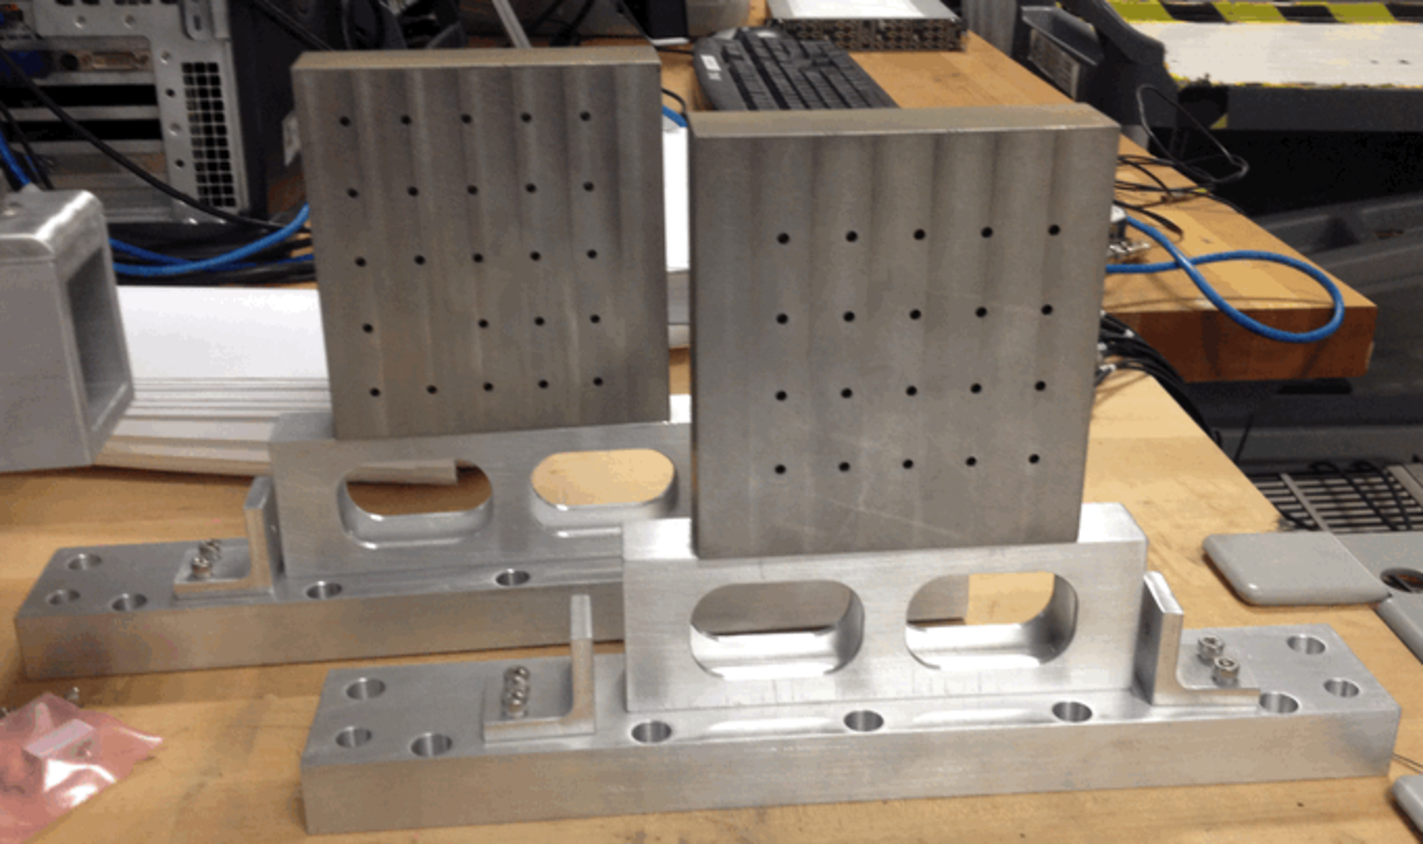
\includegraphics[width=6in]{HB_Sieve_Photo}
\caption{Upstream Sieve Slits that go on the front of the HB magnet of the SHMS \label{fig:HB_Sieve_Photo}}
\end{figure}

\begin{figure}
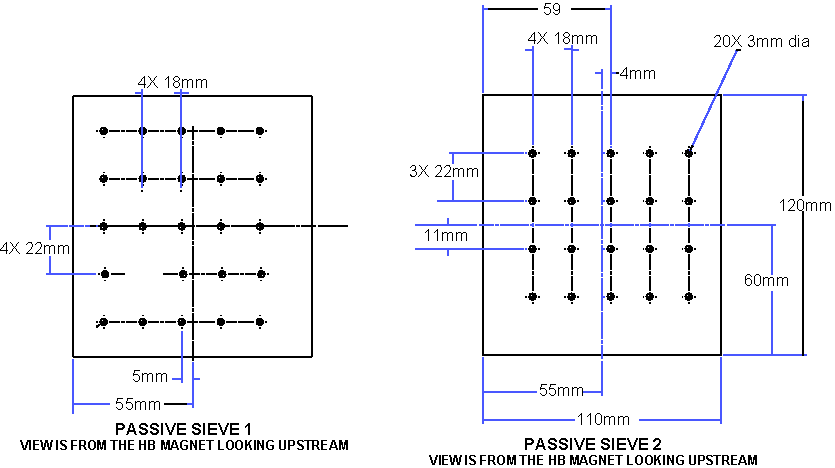
\includegraphics[width=6in]{HB_Sieve_Layout}
\caption{Upstream Sieve Slits that go on the front of the HB magnet of the SHMS \label{fig:HB_Sieve_Layout}}
\end{figure}

\subsection{Operation of the Slit System}\label{sssec:slit_control}
The HMS and SHMS slit systems are controlled by a remote control system consisting of
motor/actuators that slide the slits in place. Resolvers specify the exact position of the slits.
The resolver position of the slits is relative number of counts from the home position. The home position
is set by a homing procedure that is programmed into the controller that sets the zero position by moving the
slit to a position that activates the physical home switch. Once this homing procedure is complete, then
the slits can be moved to surveyed positions that have been programmed. The home position for HMS and SHMS slit system
does not mean that the slits are moved out of the way. For the HMS is is possible to move the slits so that
they are out of the way ({\it All Out}), but for the SHMS there is no such position for the slits.
EPICS drivers have been written for
normal operation of the slits by users and non-experts and operation of the slits through the EPICS
screens is described below. Upper and lower limit switches are on the slit system drive shaft to keep the
slits from being moved too far in either direction. There are also software limits.
The control box is located downstairs in Hall C. In the control box, there is a driver
for the HMS and one for the SHMS. If power is lost to the control box, then the brake engages
on the motor that drives the slits. On the front of the control box is
a red  emergency power shutoff button. The control box should only be opened by trained experts.

EPICS drivers have been written for normal operation of the slits by users and non-experts. The
EPICS screens are accessed through the accelerator {\bf jmenu}. Instructions for access the
  {\bf jmenu} will be given in the Hall C How-tos.
From the  {\bf jmenu}, the HMS and SHMS slit system EPICs controls can be accessed on The Hall C Operations Menu
which is open from {\bf jmenu $\rightarrow$ Standalone Menus $\rightarrow$ HallC}. On the Hall C Operations Menu under
{\it Experiment Specific} are {\it HMS Coll. Motion Control} and {\it SHMS Coll. Motion Control}. Clicking the
respective title will bring up the EPICS screens shown in Fig.~\ref{fig:normal-coll-epics}.  Fig.~\ref{fig:normal-coll-epics}
shows the HMS and SHMS slit controls in normal operation. In normal operation, the homing procedure has been completed
as indicated by the orange rectangles next to {\it Home position found/reference point point set} and {\it Home routine finished}.
With the homing procedure completed, the user can moved to the other slit positions by clicking on the labeled button. For the
HMS slit system, the slits can be moved so that they are out of the acceptance by clicking on the {\it All Out} button.
It is not possible to move the SHMS slit out of the acceptance.
\begin{figure}
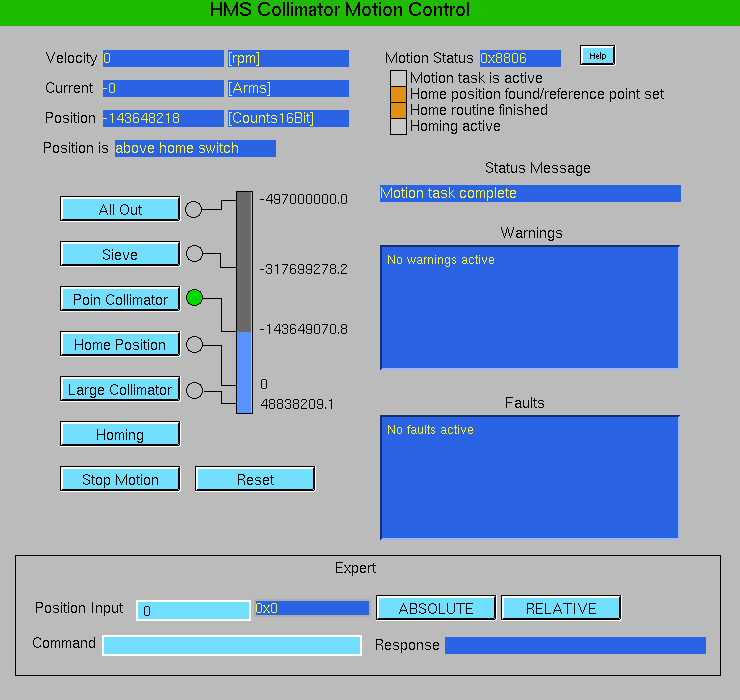
\includegraphics[width=.45\textwidth]{HMS_EPICS_pioncoll}
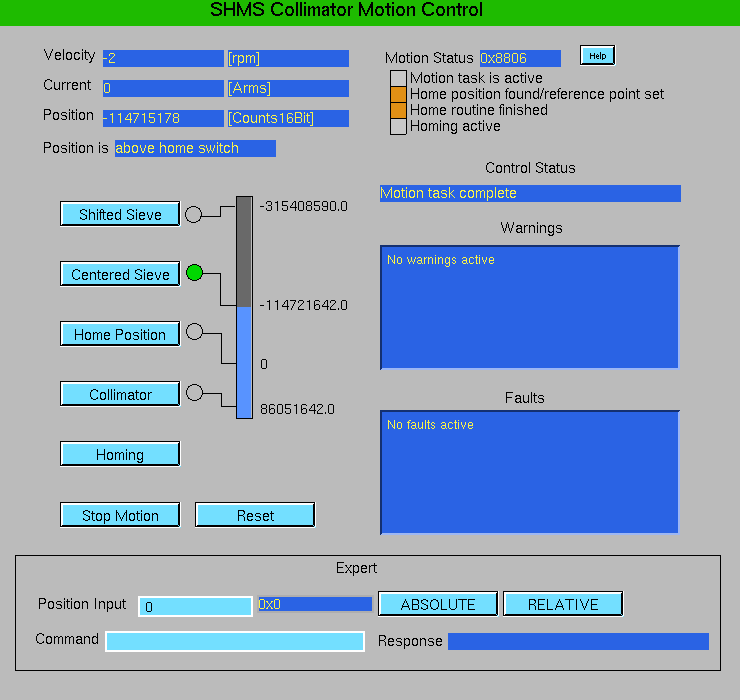
\includegraphics[width=.45\textwidth]{SHMS_EPICS_centersieve}
\caption{HMS and SHMS slit system screens in normal operation. \label{fig:normal-coll-epics}}
\end{figure}
In Fig.~\ref{fig:moving-coll-epics}, the EPICS screens are show when the slits are moving. The velocity should be around 1000 rpm and
the current less than 2 amps ( typically the reading fluctuates between 0 and 1). If the current is above 2 amps,
then click the {\it Stop Motion} button and contact the expert.
\begin{figure}
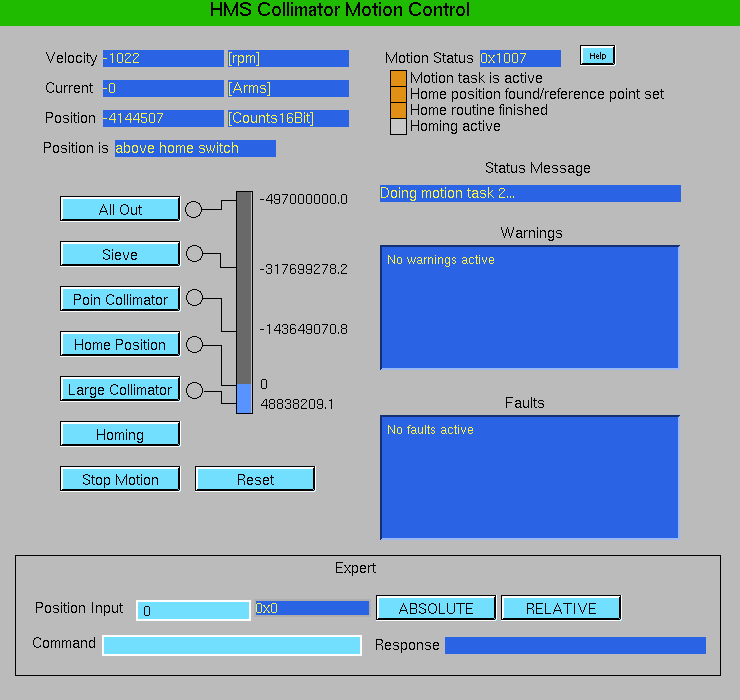
\includegraphics[width=.45\textwidth]{HMS_EPICS_moving}
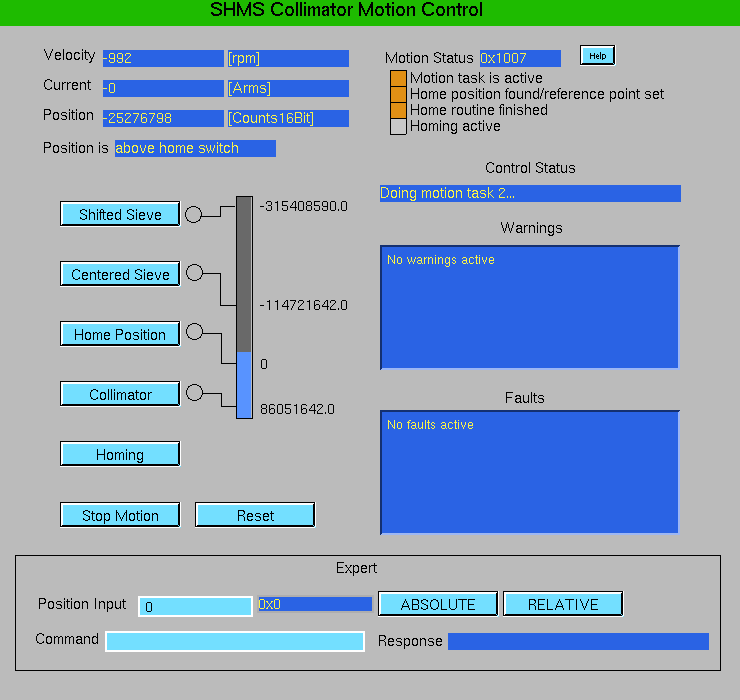
\includegraphics[width=.45\textwidth]{SHMS_EPICS_moving}
\caption{HMS and SHMS slit system screens when the slits are moving. \label{fig:moving-coll-epics}}
\end{figure}
The option of experts moving the slits to an arbitrary position
is available for the EPICS screen. The conversion is 327680 counts is one mm. The mostly likely use for this option is during the
taking of optics data when one wants data with the sieve slit moved by half the distance between holes to get more vertical angles.

The EPICS controls are done through an soft IOC called {\it  iocsofthmsco} and {\it iocsoftshmsco}. If EPICS screens are white then the IOC
needs to be rebooted. Another reason that soft IOC would need to be reboot would be if the soft IOC has lost communication with the driver.
In the case , the user could not move the slit and the text on the Warnings and Faults windows is in light grey color. Only the MCC operator can
reset the soft IOCs by accessing {\bf jmenu $\rightarrow$ Operations $\rightarrow$ Control Systems $\rightarrow$ Reboot $\rightarrow$ HallC}. The user can
call MCC to reset the soft IOCs.

If there is a power outage, the brakes are engaged in the motor that drives the slits. Once power is restored then the user needs to do the
following steps to get the slit system back in normal operation mode.
\begin{enumerate}
\item Ask MCC to reboot the soft IOC for the HMS and SHMS, {\it  iocsofthmsco} and {\it iocsoftshmsco}.
\item Access the HMS and SHMS EPICS screens.
\item On the EPICS screens, click on the {\it Reset} button. this runs an initialization program which loads parameters into the driver. The EPICS screen should look like Fig.~\ref{fig:red-screen-epics}. The red warning is to remind the user to execute the homing procedure.
\item On the EPICS screens, click on the {\it Homing} button. This executes the homing program which defines the home position and is needed before moving to other position.
\item When the homing procedure is successful then the rectangles next to {\it Home position found/reference point point set} and {\it Home routine finished} will be orange.
\item Click on button to move slit to desired position.
\end{enumerate}
\begin{figure}
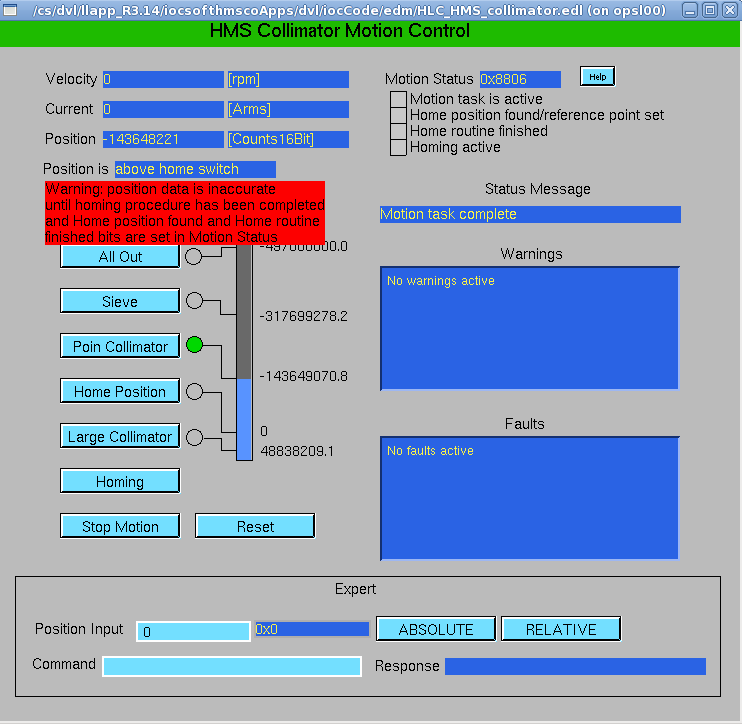
\includegraphics[width=.45\textwidth]{HMS-EPICS-red-screen}
\caption{HMS EPICS screen when power restore but before the homing procedure as been executed. \label{fig:red-screen-epics}}
\end{figure}





%\begin{table}[!ht]\
%\caption{Slit Collimator Positions\label{tab:col_pos}}
%\begin{center}
%\begin{tabular}{rlrr}
%   &                  &     HMS   & SOS\\
%\hline
%1) & Sieve Slits      &  19804600 &  11638719\\
%2) & Large Collimator &       N/A &   3190717\\
%3) & Pion Collimator  &  -3096800 &       N/A\\
%\end{tabular}
%\end{center}
%\end{table}



\subsection{Hazard Identification}

The principal hazards are:
\paragraph{Magnetic:} There is a significant fringe field at
the entrance and exits of the magnets. This represents a hazard
to people working on the slit system if they are handling magnetic
objects (tools) or to people with pacemakers. In addition the field could erase magnetic
information storage media such as the strips on credit cards.
\paragraph{Mechanical:} At the front of Q1 the housing for a spring loaded gate valve is
mounted. In its normal operation mode a metal gate will be closed with
severe pressure when the electrical power drops. This can cause serious
damage to interfering body parts.  But currently the shutter and
actuator have been removed so this hazard does not exist.
A similar mechanical problem involves the slit ladder itself. The total weight of
the three slits amounts to approximately 350 Lbs (160 Kg) and can easily
cause serious damage to body parts.

\subsection{Hazard Mitigation}

\paragraph{Magnetic}

A sign will be posted which indicates the presence of a high magnetic
field ( this is standard JLab safety signage). The exact wording is
`` High Magnetic Field - No Pacemakers or Credit Cards." There are also
flashing red lights located on the HMS and SHMS carriage indicating that the
magnet power supplies are energized. Be careful with tools (are they magnetic?)
when you work on the slit boxes with the red lights in a flashing state.

\paragraph{Mechanical}

If the gate valve is ever re-installed, the following safety
procedures should be observed.  Without power, the gate valve assumes its default closed position due to
pressured air. When installing the slit boxes, or working with your hands
in the vicinity of the inside of the gate valve, disconnect first the power
plug of the gate valve, such that the gate valve closes.
In case you need the gate valve to assume a default open position without
power, first relieve the air pressure
with power on, and verify that the default position of the gate valve has
changed to ``open" by removing the power.

When installing the slit ladder, be careful when you work with your hands
under the slit ladder (like when you are bolting the slit box to the
gate valve). Remove the slit ladder, or {\bf install a support under the slit
ladder to prevent it from falling all the way down}.

A brake system has been included in the control to prevent the slit ladder
from sliding down in case of a power failure.  However, this must not
be relied upon for personnel safety.

